\begin{lstlisting}
5.1 7 9
5.2 7 18
5.3 11 12
\end{lstlisting}
\begin{figure}[H]
\centering
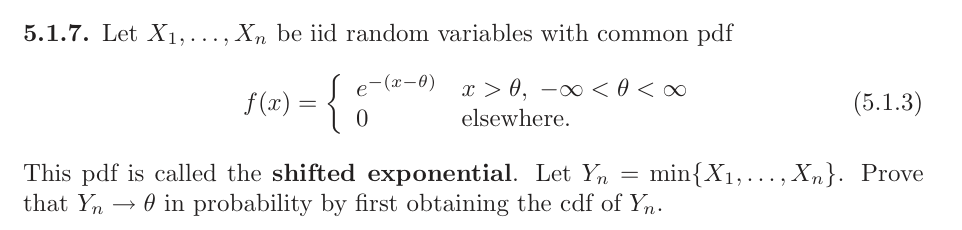
\includegraphics[width=\textwidth]{hw3-20250313.png}
% \caption{}
\label{}
\end{figure}

For
\[
\begin{aligned}
F_{Y_n}(y) & =P(Y_n\leq y)=1-P(Y_n>y)=1-P(\min\{ X_1,\dots,X_n \}>y) \\
 & =1-P(X_i>y;i=1,2,\dots,n)=1-\prod_{i=1}^{n} (1-P(X_i\leq y)) \\
 & =1-\prod_{i=1}^{n} (1-F_{X_i}(y))
\end{aligned}
\]
If $y\leq\theta$ then $F_{X_i}(y)=\int_{-\infty}^{y} f(x) \, dx=0$ thus $F_{Y_n}(y)=1-\prod_{i=1}^{n}(1-0)=0$.
If $y>\theta$ then
\[
F_{Y_n}(y)=1-\prod_{i=1}^{n} \left( 1-\int_{\theta}^{y} e^{ -(x-\theta) } \, dx  \right)=1-\prod_{i=1}^{n} e^{ -(y-\theta) }=1-e^{ -n(y-\theta) }
\]
Then for any $\varepsilon>0$, we have
\[
P(\lvert Y_n-\theta \rvert \leq \varepsilon)=P(\theta-\varepsilon \leq Y_n\leq \theta+\varepsilon)=F_{Y_n}(\theta+\varepsilon)-F_{Y_n}(\theta-\varepsilon-0)=F_{Y_n}(\theta+\varepsilon)=1-e^{ -n\varepsilon }
\]
Therefore $\lim_{ n \to \infty }P(\lvert Y_n-\theta \rvert \leq\varepsilon)=\lim_{ n \to \infty }(1-e^{ -n\varepsilon })=1$, i.e. $Y_n\to\theta$ in probability.

\begin{figure}[H]
\centering
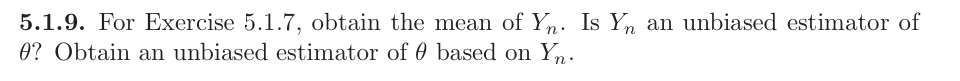
\includegraphics[width=\textwidth]{1-hw3-20250313.png}
% \caption{}
\label{}
\end{figure}
\[
p_{Y_n}(y)=F'_{Y_n}(y)=\begin{cases}
ne^{ -n(y-\theta) } & y>\theta \\
0 & y\leq \theta
\end{cases}
\]
\[
E(Y_n)=\int_{-\infty}^{\infty} yp_{Y_n}(y) \, dy =\int_{-\infty}^{\infty} y\cdot ne^{ -n(y-\theta) }\mathbb{1_{(\theta,+\infty)}}(y)  \, dy=\int_{\theta}^{+\infty } y\cdot ne^{ -n(y-\theta) } \, dy =n\theta+1
\]
Since $E(Y_n)\neq\theta$, $Y_n$ is not an unbiased estimator of $\theta$. But $Z_n=\frac{Y_n-1}{n}$ has the mean $\theta$ thus is an unbiased estimator of $\theta$.

\begin{figure}[H]
\centering
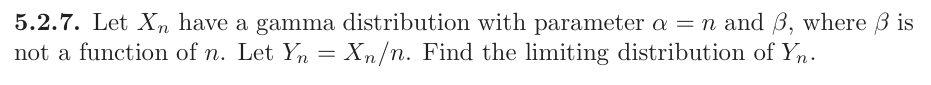
\includegraphics[width=\textwidth]{2-hw3-20250313.png}
% \caption{}
\label{}
\end{figure}

To assure the existence, we use the characteristic functions.
\[
\varphi_{X_n}(t)=E(e^{ iX_nt })=\left( 1-\frac{it}{\beta} \right)^{-n}
\]
\[
\begin{aligned}
\varphi_{Y_n}(t) & =E(e^{ iY_nt })=E(e^{ iX_nt/n  })=\varphi_{X_n}(t/n )=\left( 1-\frac{it}{n\beta} \right)^{-n} \\
 & =\exp \left\{  -n\log\left( 1-\frac{it}{n\beta} \right)  \right\}=\exp \left\{  \frac{it}{\beta}+o(1)  \right\} \\
 & \to e^{ it/\beta } \qquad \text{as }n\to \infty
\end{aligned}
\]
Denote $Y=\lim_{ n \to \infty }Y_n$.
By the inverse formula
\[
p_{Y}(x)=\frac{1}{2\pi} \int_{-\infty}^{\infty} e^{ it/\beta }\cdot e^{ -itx } \, dt=\delta_{1/\beta}(x)
\]
Then
\[
F_{Y}(x)=\begin{cases}
0 & x\leq \frac{1}{\beta} \\
1 & x> \frac{1}{\beta}  
\end{cases}
\]
\begin{figure}[H]
\centering
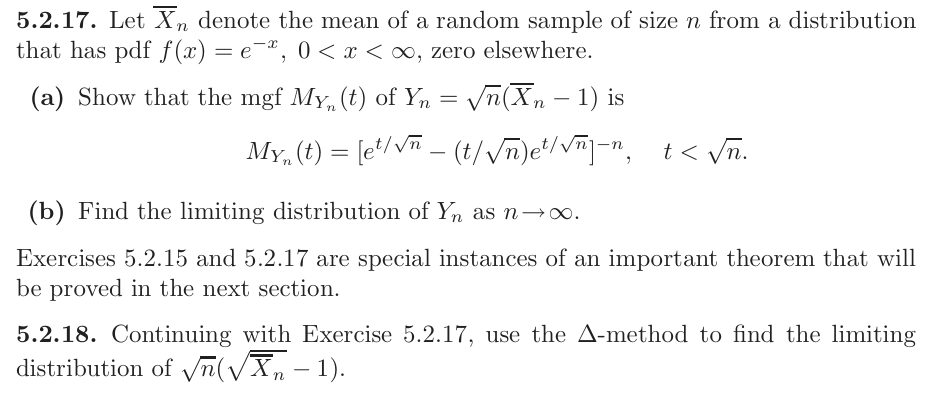
\includegraphics[width=\textwidth]{3-hw3-20250313.png}
% \caption{}
\label{}
\end{figure}
\[
\begin{aligned}
M_{Y_n}(t) & =E(e^{t \sqrt{ n }(\overline{X_n}-1) })=e^{ -t\sqrt{ n } }E\left( e^{t \frac{X_1+\dots+X_n}{\sqrt{ n }} } \right) =e^{ -t\sqrt{ n } }\prod_{k=1}^{n} E(e^{ tX_k/\sqrt{ n } }) \\
 & =e^{ -t\sqrt{ n } }\prod_{k=1}^{n} \int_{0}^{\infty} e^{ tx/\sqrt{ n } }e^{ -x } \, dx =e^{ -\sqrt{ n } }\left( \frac{1}{1-\frac{t}{\sqrt{ n }} }  \right)^{n} \\
 & =\exp \left\{  -t\sqrt{ n }-n\log\left( 1-\frac{t}{\sqrt{ n }}  \right)  \right\} \\
 & =\exp \{ -t\sqrt{ n }+t\sqrt{ n }+t^{2}/2+o(n^{-1/2 })\} \\
 & \to e^{ t^{2}/2 }\qquad \text{as }n\to \infty
\end{aligned}
\]
Denote $Y=\lim_{ n \to \infty }Y_n$, then
\[
\begin{aligned}
p_{Y}(x) & =\frac{1}{2\pi}\int_{-\infty}^{\infty} e^{ itx }M_{Y}(it) \, dt =\frac{1}{2\pi}\int_{-\infty}^{\infty} e^{ itx }e^{ -t^{2}/2  } \, dt  \\
 & =\frac{1}{2\pi}\int_{-\infty}^{\infty} e^{ -(t-ix)^{2}/2  }e^{ -x^{2}/2 } \, dt=\frac{1}{\sqrt{ 2\pi }}e^{ -x^{2}/2 }
\end{aligned}
\]
Thus $Y\sim N(0,1)$, which means
\[
Y_n=\sqrt{ n }(\overline{X}_n-1)\overset{ \mathcal{D} }{ \to }N(0,1)
\]
Let $g(x)\coloneqq \sqrt{ x }$, using the $\Delta$ -method, we have
\[
\sqrt{ n }(\sqrt{ \overline{X}_n }-\sqrt{ 1 })=\sqrt{ n }(g(\overline{X}_n)-g(1))\overset{ \mathcal{D} }{ \to }N(0,1\cdot(g'(1))^{2})=N\left( 0,\frac{1}{4} \right)
\]
Therefore the limiting distribution of $\sqrt{ n }(\sqrt{ \overline{X_n} }-1)$ is $N\left( 0,\frac{1}{4} \right)$.
\begin{figure}[H]
\centering
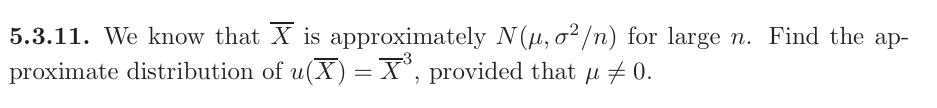
\includegraphics[width=\textwidth]{4-hw3-20250313.png}
% \caption{}
\label{}
\end{figure}

We know that
\[
\sqrt{ n }(\overline{X}-\mu)\overset{ \mathcal{D} }{ \to }N(0,\sigma^{2})
\]
Let $u(x)=x^{3}$ then $u'(x)=3x^{2}$. Using the $\Delta$ -method, we have
\[
\sqrt{ n }(u(\overline{X})-u(\mu))\overset{ \mathcal{D} }{ \to }N(0,\sigma^{2}(u'(\mu))^{2})=N(0,9\sigma^{2}\mu^{4})
\]
Therefore
\[
u(\overline{X})\overset{ \mathcal{D} }{ \to }N(\mu^{3},9\sigma^{2}\mu^{4}/n)
\]
\begin{figure}[H]
\centering
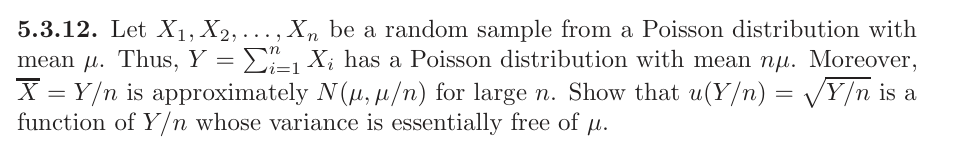
\includegraphics[width=\textwidth]{5-hw3-20250313.png}
% \caption{}
\label{}
\end{figure}

We know that
\[
\sqrt{ n }(\overline{X}-\mu)\overset{ \mathcal{D} }{ \to }N(0,\mu)
\]
Let $u(x)=\sqrt{ x }$ then $u'(x)=\frac{1}{2\sqrt{ x }}$. Using the $\Delta$ -method, we have
\[
\sqrt{ n }(u(\overline{X})-u(\mu))\overset{ \mathcal{D} }{ \to }N(0,\mu \cdot(u'(\mu))^{2})=N\left( 0,\frac{1}{4} \right)
\]
Therefore
\[
u(\overline{X})\overset{ \mathcal{D} }{ \to }N\left( \sqrt{ \mu },\frac{1}{4n}  \right)
\]
which means the variance of $\sqrt{ \frac{Y}{n} }$ is essentially free of $\mu$.
